% Fully connected neural network

\documentclass[border=10pt]{standalone}
\usepackage{tikz}
\usetikzlibrary{arrows.meta}
\tikzset{%
  >={Latex[width=2mm,length=2mm]},
  % Specifications for style of nodes:
            base/.style = {rectangle, rounded corners, %draw=black,
                           minimum width=4cm, %minimum height=1cm,
                           text centered, font=\sffamily},
         input/.style = {base, fill=green}, %green!30
         hidden/.style = {base, fill=red}, %red!30
         dropout/.style = {base, fill=orange, % orange!15
                           font=\ttfamily},
         softmax/.style = {base, fill=blue}, %blue!30
         result/.style = {base, fill=purple},  % purple!30
}
\begin{document}    
% Drawing part, node distance is 1.5 cm and every node
% is prefilled with white background
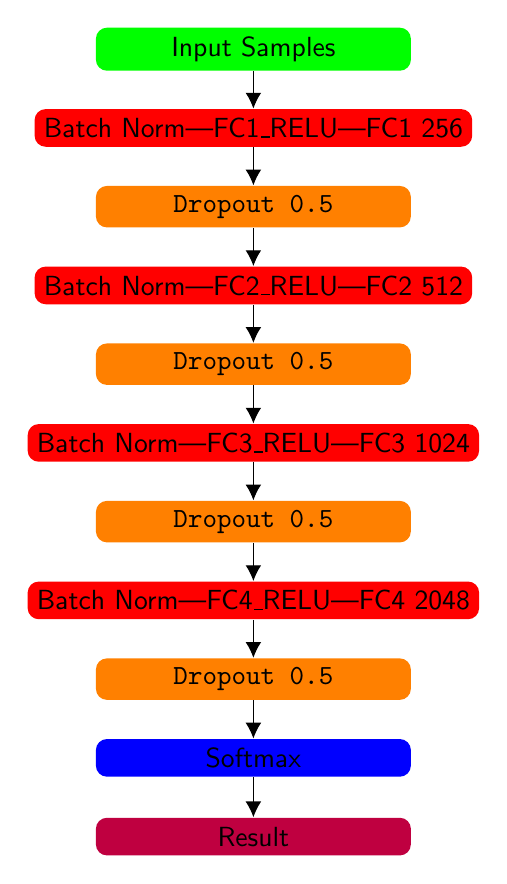
\begin{tikzpicture}[node distance=1cm,
    every node/.style={fill=white, font=\sffamily}, align=center]
  % Specification of nodes (position, etc.)
  \node (input)             [input]              {Input Samples};
  \node (hidden1)     [hidden, below of=input]          {Batch Norm|FC1\_RELU|FC1 256};
  \node (dropout1)      [dropout, below of=hidden1]   {Dropout 0.5};
  \node (hidden2)     [hidden, below of=dropout1]   {Batch Norm|FC2\_RELU|FC2 512};
  \node (dropout2)      [dropout, below of=hidden2]   {Dropout 0.5};
  \node (hidden3)     [hidden, below of=dropout2]   {Batch Norm|FC3\_RELU|FC3 1024};
  \node (dropout3)      [dropout, below of=hidden3]   {Dropout 0.5};
  \node (hidden4)     [hidden, below of=dropout3]   {Batch Norm|FC4\_RELU|FC4 2048};
  \node (dropout4)      [dropout, below of=hidden4]   {Dropout 0.5};
  
  \node (softmax)      [softmax, below of=dropout4]   {Softmax}; 
  \node (result)      [result, below of=softmax]   {Result};
%  \node (softmax)   [softmax, below of=dropout4,yshift=0.5cm]{Softmax};
%  \node (result)    [result, below of=softmax,yshift=0.5cm]{Result};    
  % Specification of lines between nodes specified above
  % with aditional nodes for description 
  \draw[->]       (input) -- (hidden1);
  \draw[->]       (hidden1) -- (dropout1);
  \draw[->]       (dropout1) -- (hidden2);
  \draw[->]       (hidden2) -- (dropout2);
  \draw[->]       (dropout2) -- (hidden3);
  \draw[->]       (hidden3) -- (dropout3);
  \draw[->]       (dropout3) -- (hidden4);
  \draw[->]       (hidden4) -- (dropout4);
  \draw[->]       (dropout4) --(softmax);
  \draw[->]       (softmax) -- (result);
  
  \end{tikzpicture}
\end{document}